\documentclass[a4paper]{article}
\usepackage[utf8]{inputenc}
\usepackage[L7x]{fontenc}
\usepackage[lithuanian]{babel}
\usepackage{lmodern}
\usepackage{amsmath}
\usepackage[top=2cm, bottom=2cm, left=2cm, right=2cm, footskip=1cm, a4paper]{geometry}

\usepackage{tasks}
\usepackage{hyperref}
\usepackage{graphicx}
\usepackage{animate}
\usepackage{tikz}
\begin{document}
\section{Integralai}
\subsection{Kas yra integralas?}
Integralu $\displaystyle \int_a^b f(x)dx$ laikomas srities tarp $Ox$ ašies ir $f(x)$ plotas, kai $x \in [a,b]$.
Intervalo $[a,b]$ kraštai (\href{dydziai.png}{\textbf{pastovieji dydžiai}}) $a$ ir $b$ yra vadinami integralo rėžiais.
\subsection{Integravimo rėžiuose iliustracija}

\newcounter{r}
\newcommand{\escalar}[1]{
\setcounter{r}{#1 * #1 * #1}
}
%
\newcounter{m}
\setcounter{m}{0}
\newcounter{mc}

\begin{animateinline}[loop, poster = first, controls, palindrome]{2}
\whiledo{\them < 21}{
    \begin{tikzpicture}[scale=1.25]
    \draw[red,thick,<->] (-1,1) parabola bend (0,0) (2.1,4.41)
        node[below right] {$y=x^2$};
    \draw[loosely dotted] (-1,0) grid (4,4);
    %\path[use as bounding box] (-2,-1) rectangle (5,5);
    \draw[->] (-0.2,0) -- (4.25,0) node[right] {$x$};
    \draw[->] (0,-0.25) -- (0,4.25) node[above] {$y$};
    \foreach \x/\xtext in {1/1, 2/2, 3/3}
    \draw[shift={(\x,0)}] (0pt,2pt) -- (0pt,-2pt) node[below] {$\xtext$};
    \foreach \y/\ytext in {1/1, 2/2, 3/3, 4/4}
    \draw[shift={(0,\y)}] (2pt,0pt) -- (-2pt,0pt) node[left] {$\ytext$};
%
    \setcounter{mc}{\value{m}*\value{m}}
    \shade[top color=blue,bottom color=gray!50]
        (0,0) parabola (0.1*\them,0.01*\themc) |- (0,0);
    \escalar{\them}
    \draw (3cm,2pt) node[above]
        {$\displaystyle\int\limits_0^{\them/10} \!\!x^2\mathrm{d}x = 
            \displaystyle\frac{\ther}{3000}$};
    \draw[fill=orange,color=orange] (0.1*\them,0.01*\themc) circle (0.5pt);
    \end{tikzpicture}
    %
    \stepcounter{m}
    \ifthenelse{\them < 21}{
            \newframe
    }{
        \end{animateinline}\relax % BREAK
    }
}
\subsection{Integravimo rėžiuose algebrinė prasmė}

\textbf{Kaip formaliai apskaičiuoti} $\displaystyle \int_a^b f(x)dx$?
\begin{itemize}
\item Sričiai $[a, b]$ imame dalą $P$, aprašomą $a=x_0 <  x_1 < x_2 < \dots < x_n=b$. 
\item Apskaičiuojame sumą $\displaystyle \sum_{i=1}^{n}f(x_i)(x_i-x_{i-1})$
\item Apskaičiuojame ribą $\displaystyle \lim_{n \to \infty} \left(\sum_{i=i}^{n}f(x_i)(x_i-x_{i-1})\right)$
\end{itemize}
Skaičiavimai daug supaprastėja, kai $x_0, x_1, x_2, ..., x_n$ yra išsidėstę vienodais atstumais. Tuomet galioja

$\begin{cases}x_0=a \\ x_1=a+\frac{1}{n} \\ x_2=a+\frac{2}{n} \\ \cdots \end{cases} \Rightarrow \begin{cases} x_1-x_0=\frac{1}{n} \\ x_2-x_1=\frac{1}{n} \\ \cdots \\ x_n-x_{n-1}=\frac{1}{n} \end{cases}$ ir telieka apskaičiuoti ribą $\displaystyle \lim_{n \to \infty} \sum_{i=1}^{n}\frac{f\left(a+\frac{i}{n}\right)}{n}$

\subsection{Uždaviniai iš integralų}
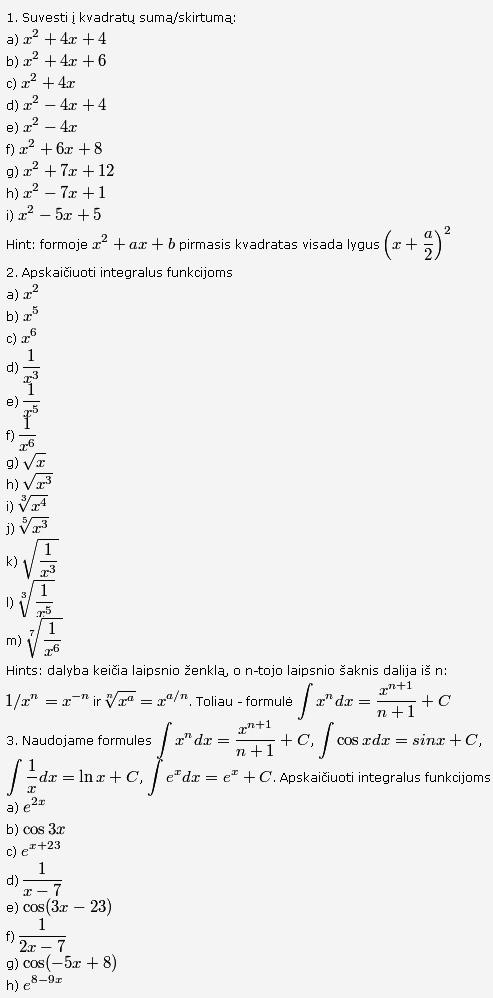
\includegraphics[width=0.67\textwidth]{int_uzd.jpg}
\newpage
\subsection{Uždavinių iš integralų atsakymai}
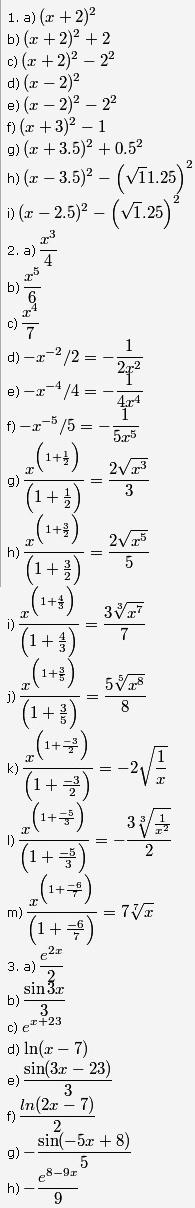
\includegraphics[width=0.23\textwidth]{int_ats.jpg}
\end{document}